\documentclass[../main.tex]{subfile}

\begin{document}

\begin{figure*}
    \centering
    \begin{minipage}{17.5cm}
        \subfloat[RGB]{
            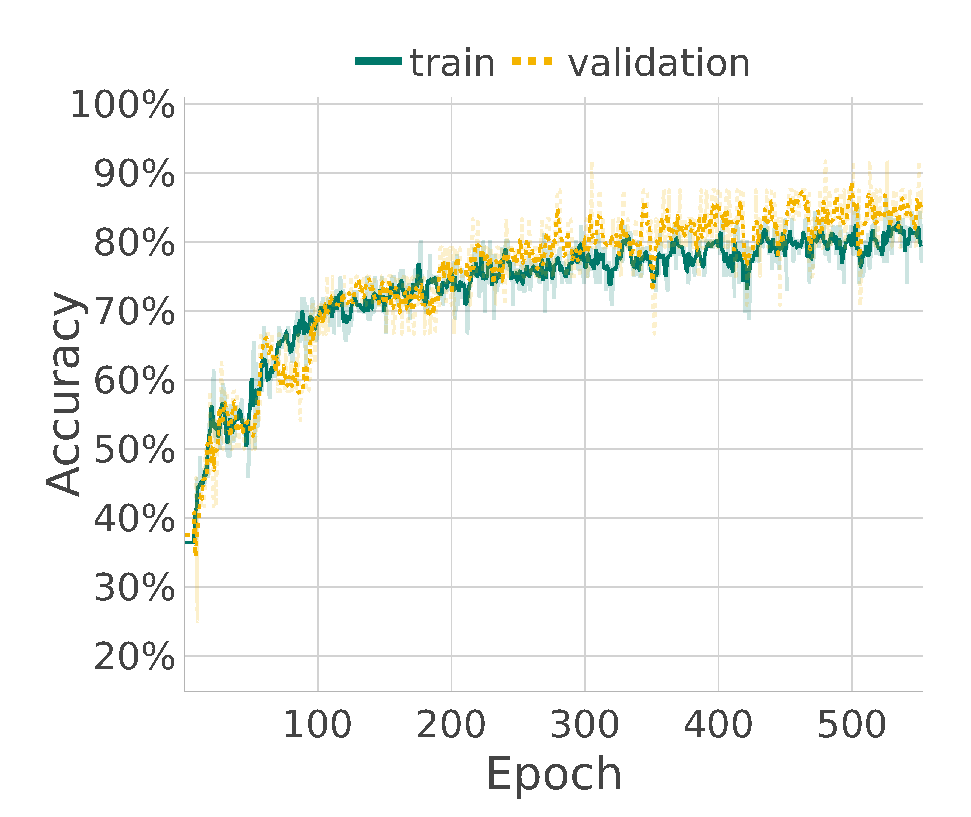
\includegraphics[width=.33\textwidth]{images/graphs/siriguela/gabor/rgb.eps}
        }
        \subfloat[Grayscale]{
            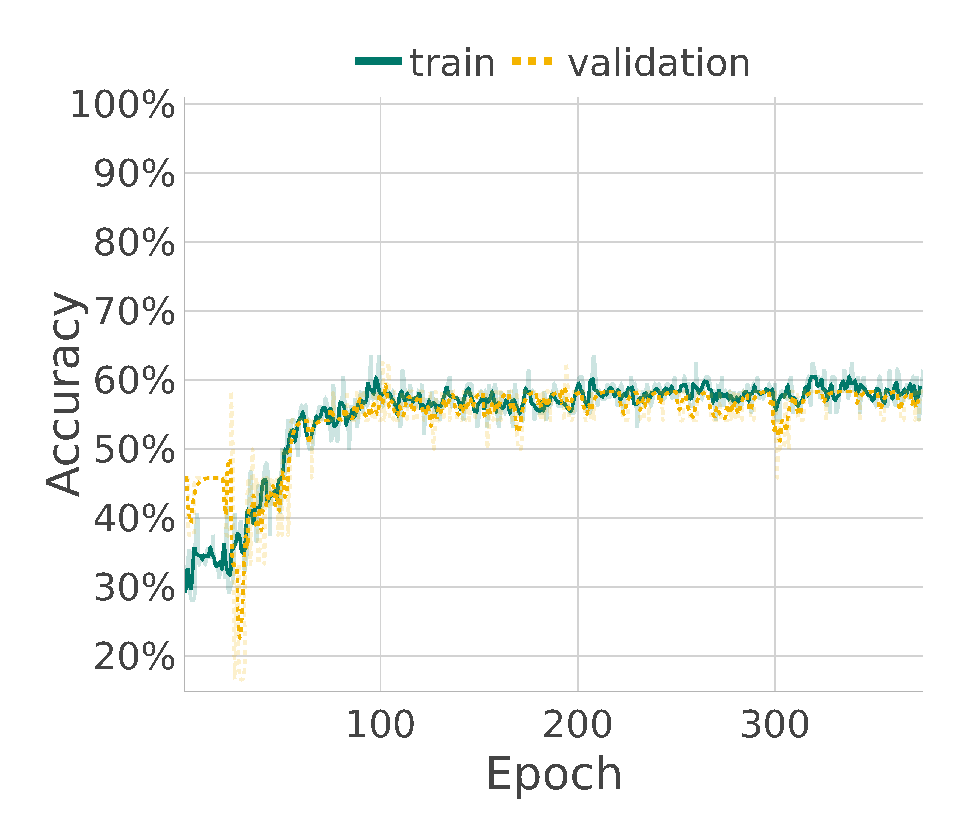
\includegraphics[width=.33\textwidth]{images/graphs/siriguela/gabor/grayscale.eps}
        }
        \subfloat[GLCM]{
            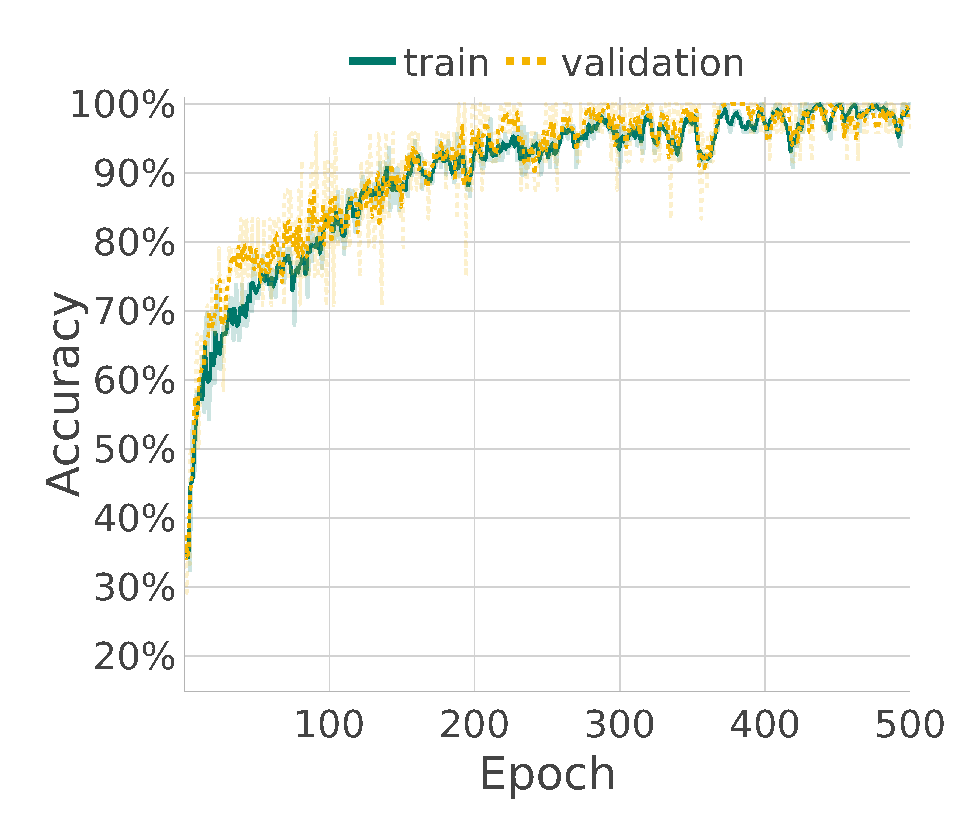
\includegraphics[width=.33\textwidth]{images/graphs/siriguela/gabor/glcm.eps}
        }

        \caption{Training curves for the models trained on \textit{siriguelas} images.} \figfooter{a}{It was used RGB images.}
        \figfooter{b}{It was used grayscale images.}
        \figfooter{c}{It was used some texture properties from a GLCM.}
        \label{fig:siriguelas}
    \end{minipage}
\end{figure*}

\end{document}